\chapter{Исследовательский раздел}
В данном разделе представлены тестовые наборы данных, примеры работы программы, замеры времени и пикового значения памяти для разного размера входных строк и для разных алгоритмов.

\section{Тестовые наборы}
В качестве демонстрации правильности работы алгоритмов протестирован набор данных, представленный в таблице \ref{tests}.

\begin{table}[H]
\caption{Тестовые наборы к реализованной программе}
\label{tests}
\begin{center}
	\begin{tabular}{|c|c|c|p{3cm}|p{3cm}|c|}
		\hline
		№ & Строка 1 & Строка 2 & Расстояние\linebreak Левенштейн & Расстояние\linebreak Дамерау-\linebreak Левенштейна & Результат\\
		\hline
		1 & & & 0 - 0 - 0 & 0 & Passed \\ 
		\hline
		2 & МГТУ & & 4 - 4 - 4 & 4 & Passed \\ 
		\hline
		3 & & Бауман & 6 - 6 - 6 & 6 & Passed\\
		\hline
		4 & скат & скот & 1 - 1 - 1 & 1 & Passed\\
		\hline
		5 & рыба & рба & 1 - 1 - 1 & 1 & Passed\\
		\hline
		6 & клавиатура & кклавиатура & 1 - 1 - 1 & 1 & Passed\\
		\hline
		7 & универ & униевр & 2 - 2 - 2 & 1 & Passed\\
		\hline
		8 & агент & ааген & 2 - 2 - 2 & 2 & Passed\\
		\hline
		9 & море & моорк & 2 - 2 - 2 & 2 & Passed\\
		\hline
		10 & солнце & соллннце & 2 - 2 - 2 & 2 & Passed\\
		\hline
		11 & трава & ртаваа & 3 - 3 - 3 & 2 & Passed\\
		\hline
		12 & ноутбук & ноубцк & 2 - 2 - 2 & 2 & Passed\\
		\hline
		13 & компьютер & кмпьюетр & 3 - 3 - 3 & 2 & Passed\\
		\hline
		14 & экран & эан & 2 - 2 - 2 & 2 & Passed\\
		\hline
		15 & мышка & мфшак & 3 - 3 - 3 & 2 & Passed\\
		\hline
		16 & пиксель & пиесмль & 2 - 2 - 2 & 2 & Passed\\
		\hline
		17 & интернет & нитерент & 4 - 4 - 4 & 2 & Passed\\
		\hline
		18 & данные & ддннеы & 3 - 3 - 3 & 2 & Passed\\
		\hline
		19 & диспетчер & дииспечео & 3 - 3 - 3 & 3 & Passed\\
		\hline
		20 & алгоритм & агоиртс & 4 - 4 - 4 & 3 & Passed\\
		\hline
	\end{tabular}
\end{center}
\end{table}
В результате тестрования все тесты пройдены успешно, что показывает правильность работы алгоритма на различных строках.

\section{Примеры работы программы}
На рисунках \ref{example_1} - \ref{example_2} представлены примеры работы программы.

\begin{minipage}{.49\textwidth}
	\centering
	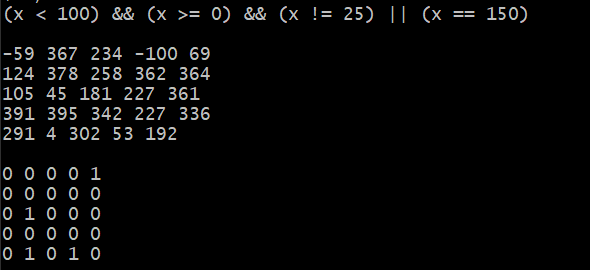
\includegraphics[scale=0.6]{inc/img/example_1.png}
	\captionof{figure}{Пример работы №1}
	\label{example_1}
\end{minipage}
\begin{minipage}{.49\textwidth}
	\centering
	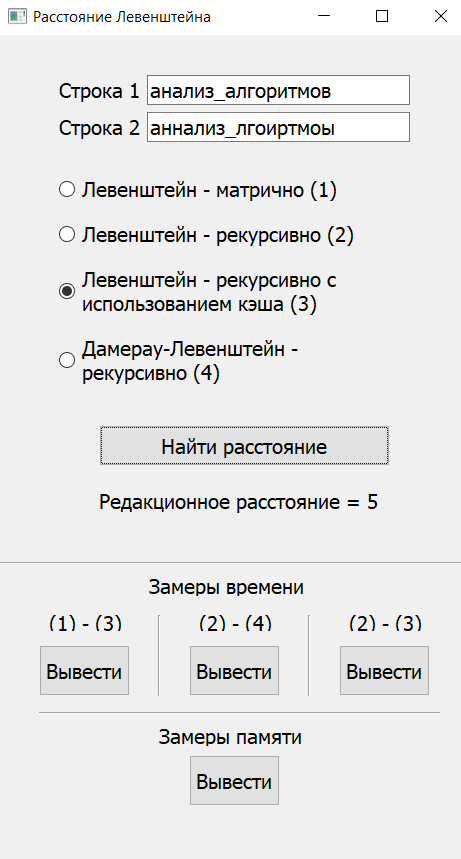
\includegraphics[scale=0.6]{inc/img/example_2.png}
	\captionof{figure}{Пример работы №2}
	\label{example_2}
\end{minipage}

\section{Время выполнения алгоритмов}
Как упоминалось ранее для сравнения эффективности алгоритмов используются стандартные библиотеки time и functools. 

Разработанная программа предоставляет интерфейс, позволяющий пользователю получить зависимости времени выполнения алгоритма от размера строки для различных пар: 1) Левенштейн (матрично) - Левенштейн (рекурсивно с использованием кэша)); 2) Левенштейн (рекурсивно) - Дамерау-Левенштейн (рекурсивно); 3) Левенштейн (рекурсивно) - Левенштейн (рекурсивно с использованием кэша). Соответствующие графики которых изображены на рисунках \ref{graph_1} - \ref{graph_3}.

\begin{figure}[p]
	\center{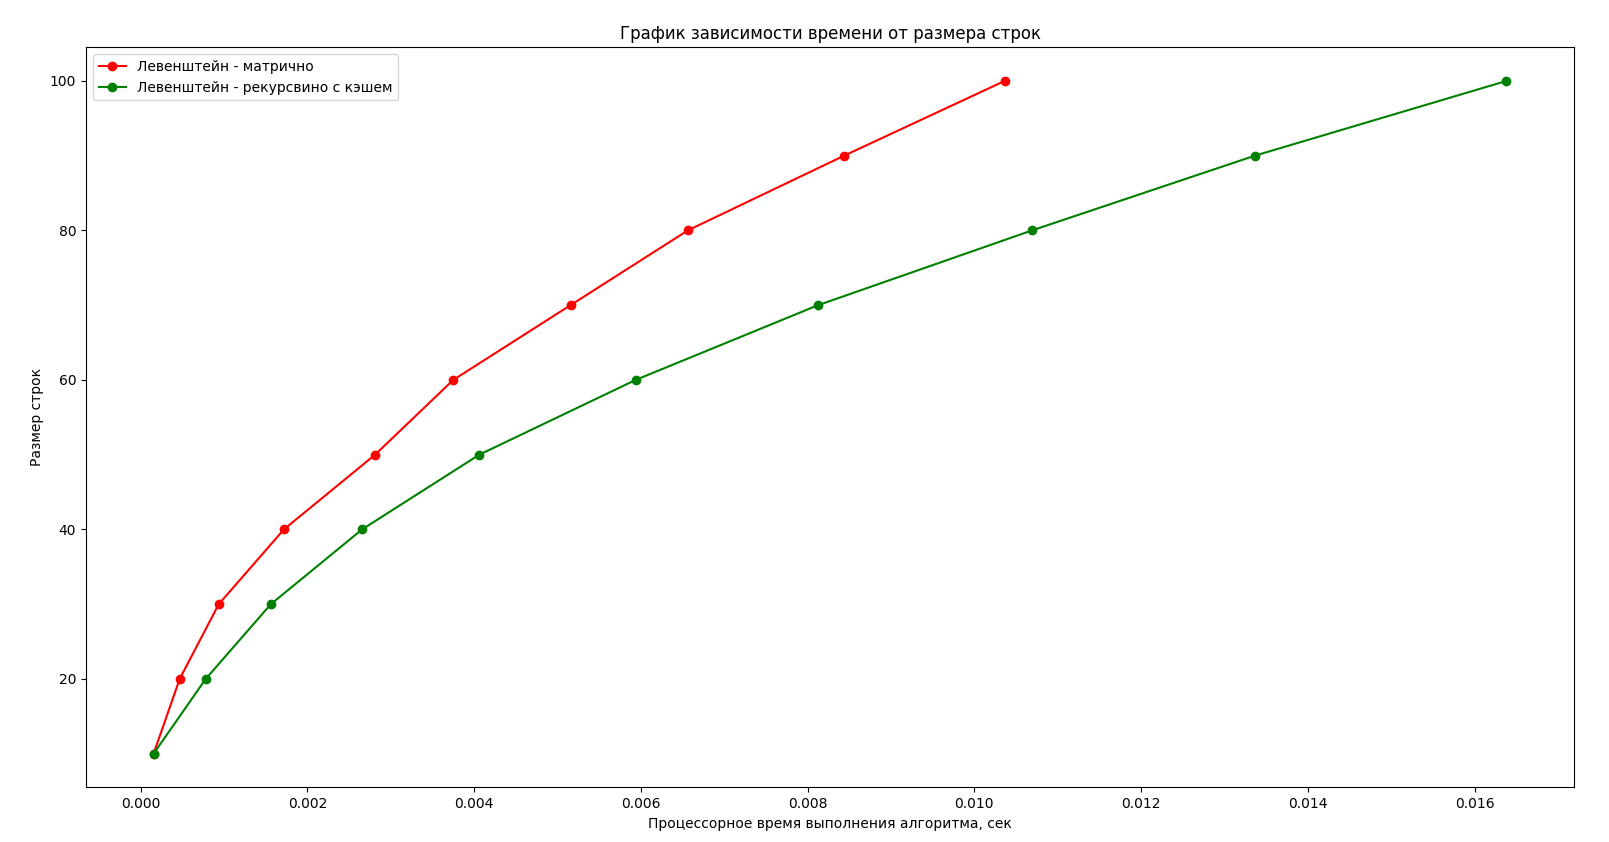
\includegraphics[scale=0.42]{inc/img/graph_1.png}}
	\caption{Зависимости времени работы алгоритмов поиска расстояния Левенштейна матричным способом и рекурсивным с использованием кэша от размера строк}
	\label{graph_1}
\end{figure}
\begin{figure}[p]
	\center{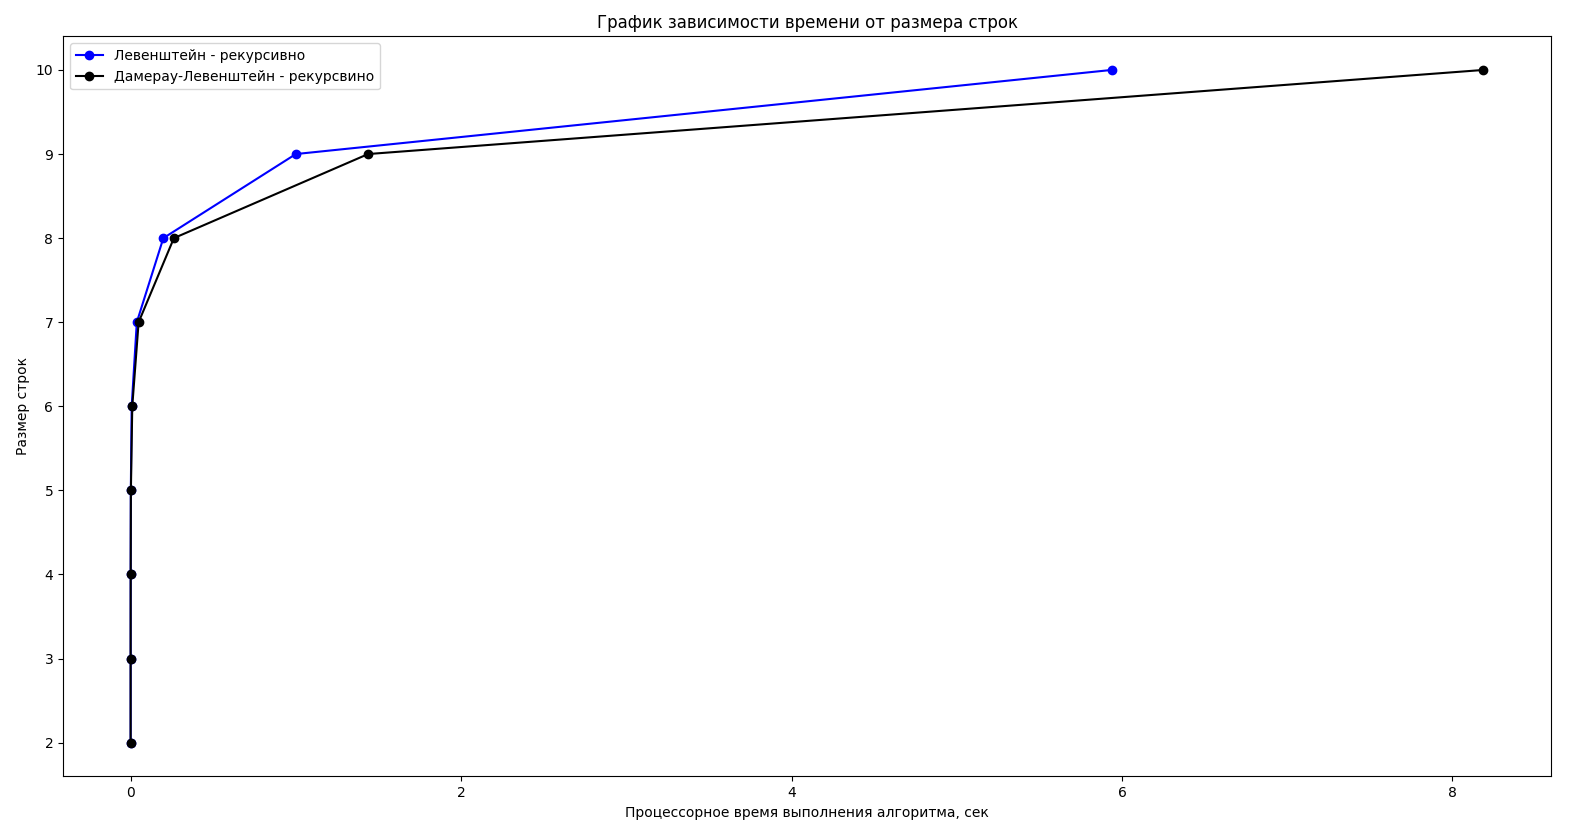
\includegraphics[scale=0.42]{inc/img/graph_2.png}}
	\caption{Зависимости времени работы алгоритмов поиска расстояний Левенштейна и Дамерау-Левенштейна рекурсивно от размера строк}
	\label{graph_2}
\end{figure}
\begin{figure}[h]
	\center{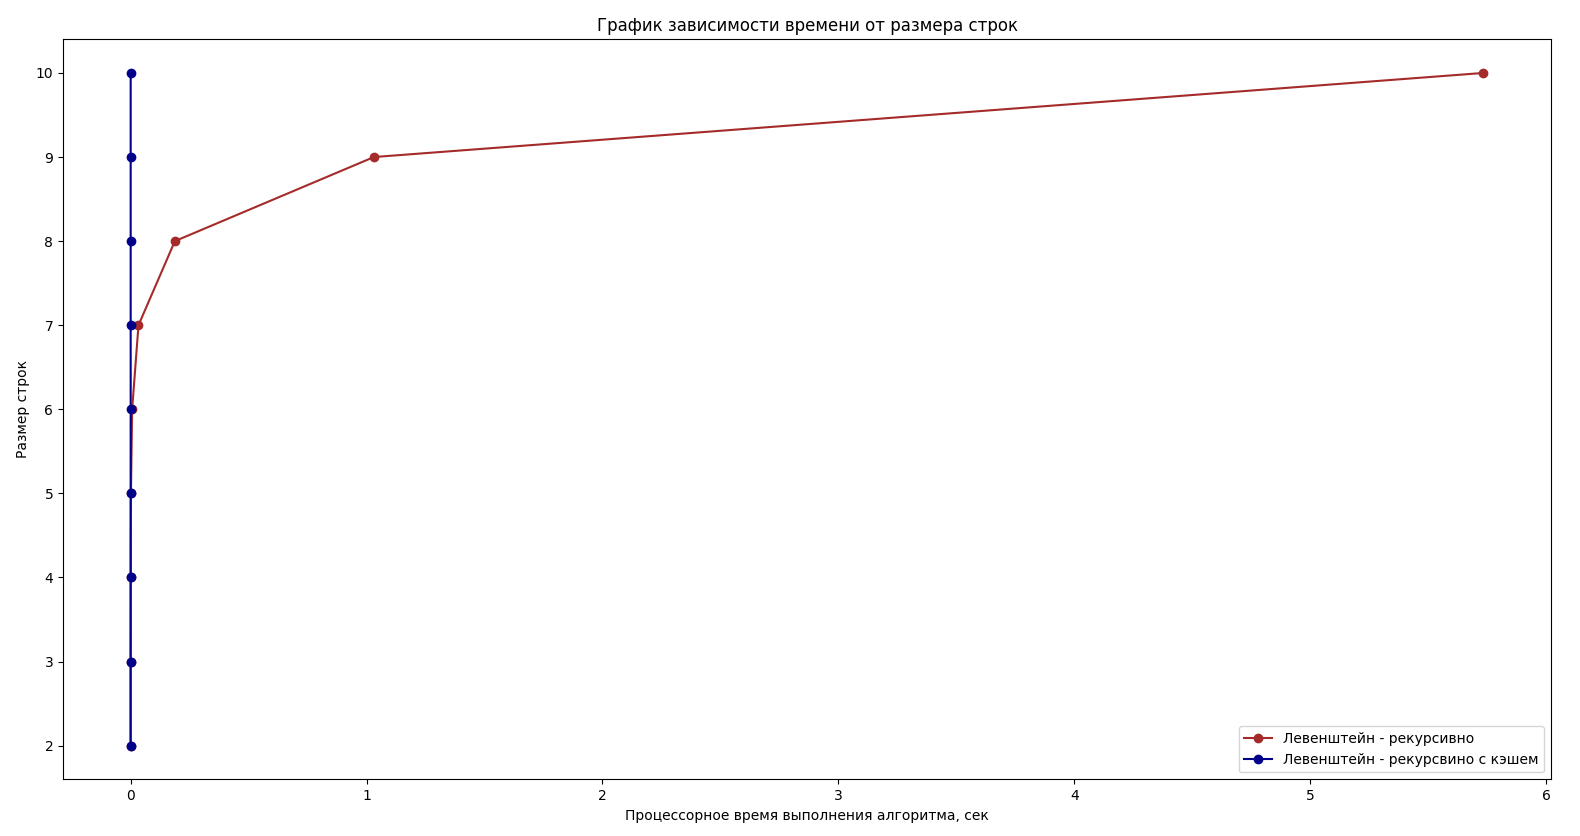
\includegraphics[scale=0.42]{inc/img/graph_3.png}}
	\caption{Зависимости времени работы алгоритмов поиска расстояния Левенштейна рекурсивно с использованием кэша и без от размера строк}
	\label{graph_3}
\end{figure}
\newpage
Из рисунка \ref{graph_1} видно, что матричный способ и рекурсивный с использованием кэширования являются достаточно эффективными по времени ($\sim$(0.1 - 0.2) секунды на обработку строк длинами 100), при этом на всех длинах использование матрицы показывает лучший результат (в $\sim$1.5 раза). Рекурсивные реализации алгоритмов нахождения расстояний Левенштейна и Дамерау-Левенштейна (рисунок \ref{graph_2}) долго производят обработку строк - время растет геометрически. Ожидаемо, что для расстояния Дамерау-Левенштейна медленней, так как требуется больше действий. Рисунок \ref{graph_3} показывает, какое преимущество дает использование кэширования при рекурсивной реализации. Видно, что в таком случае значения колеблются в пределах 0, тогда как для обычной версии при размере строк 10 тратится $\sim$6 секунд.

\section{Пиковое значение памяти}
На рисунке 

\section{Вывод}